\chapter{Learned Probabilistic Sun Sensor}
\epigraph{He stepped down, avoiding any long look at her as one avoids long looks at the sun, but seeing her as one sees the sun, without looking.}{Leo Tolstoy, \textit{Anna Karenina}}
\label{ch:sun-bcnn}


\section{Background}
\subsection{Regularization and Dropout}
Recall from \Cref{section:math_dl_practical} that dropout (\Cref{fig:sun-bcnn_dropout}) was originally proposed as a regularization technique that improves the generalization performance of deep networks.

\subsection{Bayesian Modelling and Variational Inference}

Our goal is to generate a function $f(\Vector{x}; \GenericParameters)$ that maps inputs $\Vector{x}$ to outputs $\Vector{y}$ a function of parameters $\GenericParameters$. Recall from \Cref{ch:probe}, that in Bayesian inference, we define a \textit{prior} on the space of parameters $p(\GenericParameters)$ and a \textit{likelihood function} that defines how likely we are to observe $\Vector{y}$ given an input $\Vector{x}$ and parameters $\GenericParameters$, $p(\Vector{y} | \Vector{x}, \GenericParameters)$. For example for regression problems, we may define the likelihood
\begin{equation}
	p(\Vector{y} | \Vector{x}, \GenericParameters) = \NormalDistribution(f(\Vector{x}; \GenericParameters),\tau^{-1}\IdentityMatrix)
\end{equation}
where $\tau$ is a model \textit{precision}. Given a dataset $\mathcal{D} = \{\Matrix{X}, \Matrix{Y}\} = \{\{\Vector{x}_1, ... \Vector{x}_N\},\{\Vector{y}_1, ..., \Vector{y}_N)\} \}$, the Bayesian formulation seeks a posterior over the parameters $\GenericParameters$:
\begin{equation}
\label{eq:sun_bcnn_param_posterior}
	p(\GenericParameters | \mathcal{D}) = \frac{p(\Matrix{Y}|\Matrix{X}, \GenericParameters) p(\GenericParameters)}{p(\Matrix{Y} | \Matrix{X})}
\end{equation}
where we may think of this posterior as evaluating the sentence `the likelihood of the observed outputs given a particular set of parameters (weighed by a prior) compared to how likely they are in general'. This latter `in general' quantity is the marginal likelihood (also known as the model \textit{evidence}) over the space of parameters,
\begin{equation}
	p(\Matrix{Y} | \Matrix{X}) = \int_{\GenericParameters}  p(\Matrix{Y} | \Matrix{X}, \GenericParameters) p(\GenericParameters) d\GenericParameters.
\end{equation}
For a given test input $\Vector{x}^*$, we can then \textit{infer} a predictive distribution over the space of outputs by integrating over the posterior of model parameters:
\begin{equation}
	p(\Vector{y}^* | \Vector{x}^*, \mathcal{D}) = \int_{\GenericParameters}  p(\Vector{y}^* | \Vector{x}^*, \GenericParameters) p(\GenericParameters | \mathcal{D}) d\GenericParameters.
\end{equation}
For most problems, evaluating the posterior (\Cref{eq:sun_bcnn_param_posterior}) analytically is not problems. Instead, we can employ the technique of \textit{variational inference} \citep{Gal2016UncertaintyThesis}.

\subsubsection{Variational Inference}
In variational inference, we define a simpler variational density $q(\GenericParameters; \Vector{\theta})$ based on the auxiliary parameters $\Vector{\theta}$. We then seek to minimize the Kullback-Leibler (KL) divergence between $q(\GenericParameters; \Vector{\theta})$ and the true posterior $p(\GenericParameters | \mathcal{D})$:
\begin{equation}
\label{eq:sun_bcnn_KL}
	\Vector{\theta}^* = \ArgMin{\Vector{\theta}}\text{KL}(q(\GenericParameters; \Vector{\theta}) || p(\GenericParameters | \mathcal{D})),
\end{equation}
which then allows us to compute the approximate predictive distribution as
\begin{equation}
	p(\Vector{y}^* | \Vector{x}^*, \mathcal{D}) \approx \int_{\GenericParameters}  p(\Vector{y}^* | \Vector{x}^*, \GenericParameters) q(\GenericParameters; \Vector{\theta}^*) d\GenericParameters.
\end{equation}
One can show that minimizing KL divergence (\Cref{eq:sun_bcnn_KL}) is the same as maximizing the evidence lower bound (ELBO)\footnote{KL divergence and the ELBO differ by a constant that is not dependent on the auxiliary variables.} 
\begin{equation}
\label{eq:sun_bcnn_ELBO}
	\Vector{\theta}^* = \ArgMax{\Vector{\theta}} \int_{\GenericParameters}  \log p(\Matrix{Y} | \Matrix{X}, \GenericParameters)  q(\GenericParameters; \Vector{\theta}) d\GenericParameters -  \text{KL}(q(\GenericParameters; \Vector{\theta}) ~ || ~ p(\GenericParameters)).
\end{equation}
Intuitively, maximizing the first term above (referred to as the expected log likelihood) ensures that $q(\GenericParameters; \Vector{\theta})$ explains the dataset well, while minimizing the latter term regularizes the optimization so that $q(\GenericParameters; \Vector{\theta})$ does not stray too far away from a prior.

\begin{figure}
\centering
\begin{subfigure}{0.45\textwidth}
	\centering
    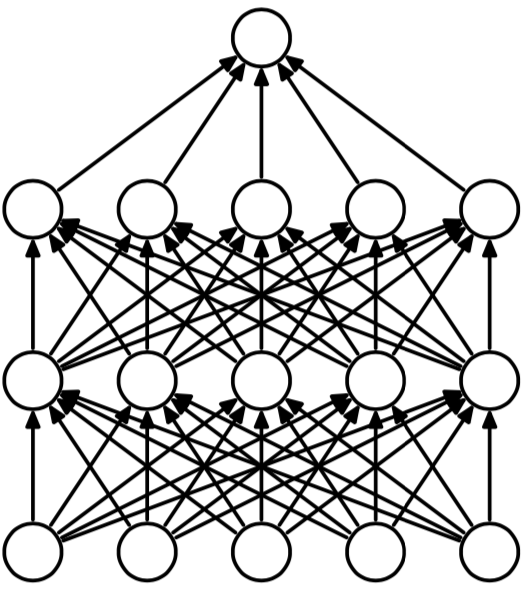
\includegraphics[width=0.8\textwidth]{sun-bcnn/dropout_fcn}
    \caption{Standard fully-connected neural network.}
\end{subfigure}
~
\begin{subfigure}{0.45\textwidth}
	\centering
    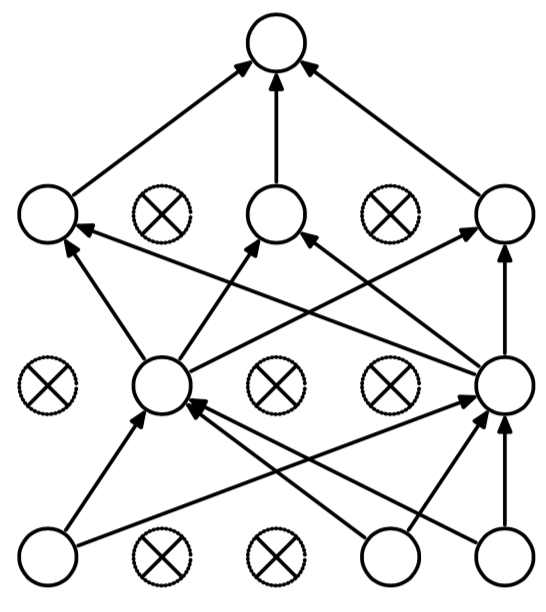
\includegraphics[width=0.8\textwidth]{sun-bcnn/dropout_fcnwdrop}
    \caption{A neural network with dropout applied.}
\end{subfigure}
\caption{The technique of \textit{dropout} stochastically removes the contribution of certain neurons to regularize learning. Figures	 from \cite{srivastava_dropout_2014}.}
\label{fig:sun-bcnn_dropout}
\end{figure}



\subsection{Monte Carlo Dropout as Approximate Variational Inference}
A key insight of Bayesian Neural Networks \citep{Gal2016UncertaintyThesis, Gal2016-ny} is the training objective of a neural network with dropout resembles the ELBO optimization of \Cref{eq:sun_bcnn_ELBO} with a careful choice of $q(\GenericParameters; \Vector{\theta})$ such that a particular condition holds (Eq. 3.12, \cite{Gal2016UncertaintyThesis}).

Namely, consider training a neural network with dropout and with \textit{weight decay} (as is commonly done). The loss function for supervised training in this scenario can be written as
\begin{equation}
\mathcal{L}_{\text{dropout}}(\GenericParameters) = \underbrace{\frac{1}{N} \sum_{i=1}^N \mathcal{E}(\Vector{y}_i, \tilde{\Vector{y}}_i)}_{\text{error function}} + \underbrace{\lambda \sum_{\ell=1}^L	\left( \Norm{\Matrix{W}_\ell}_2^2 +  \Norm{\Vector{b}_\ell}_2^2\right)}_{\text{weight decay}},
\end{equation}
where $\Vector{y}_i$ is the target output and $\tilde{\Vector{y}}_i = NN(\Vector{x}_i)$ is a stochastic sample of the network output.

Now consider that we define our auxiliary parameters for $q$ to be the neural network weight matrices, $\Vector{\theta} = \{\Matrix{W}_\ell\}_{\ell=1}^L$, and treat the parameters of
\begin{align}
	q(\GenericParameters; \Vector{\theta}) &= \text{diag} (\{ b_{i\ell} \}) \Matrix{W}_\ell \\
	b_{i\ell} &\sim \text{Bernoulli}(p_i) 
\end{align}

Namely we can use a stochastic estimator such that:

\begin{align}
		p(\Vector{y}^* | \Vector{x}^*, \mathcal{D}) &\approx \int_{\GenericParameters}  p(\Vector{y}^* | \Vector{x}^*, \GenericParameters) q(\GenericParameters; \Vector{\theta}^*) d\GenericParameters \\
		&\approx \frac{1}{T} \sum_{t=1}^T p(\Vector{y}^* | \Vector{x}^*, \tilde{\GenericParameters}_t)
\end{align}
where $\tilde{\GenericParameters}_t$ is a sample of our trained network with dropout applied at test time.



